\author{Adrien Ferreira, Alexandra Hospital}

\institute{PSAR - UPMC}

\date{26 mars 2015}



% ****************** Page de garde ******************
\begin{document}

   \begin{frame}

      \titlepage

   \end{frame}


% ******************** Table des matieres ********************
%  S'ajoute à chaque fin de section pour montrer 
%  où on est dans la présensation 

\AtBeginSection[]
{
\begin{frame}

     \frametitle{Sommaire}

        \tableofcontents[currentsection]

\end{frame} 
}


% ************ Présentation du projet ************ 

\section{Présentation du projet}

	% *** Balezator en ligne ***
	\subsection{Balezator en ligne}

	\begin{frame}

		\frametitle{Lecture sur le manche}
			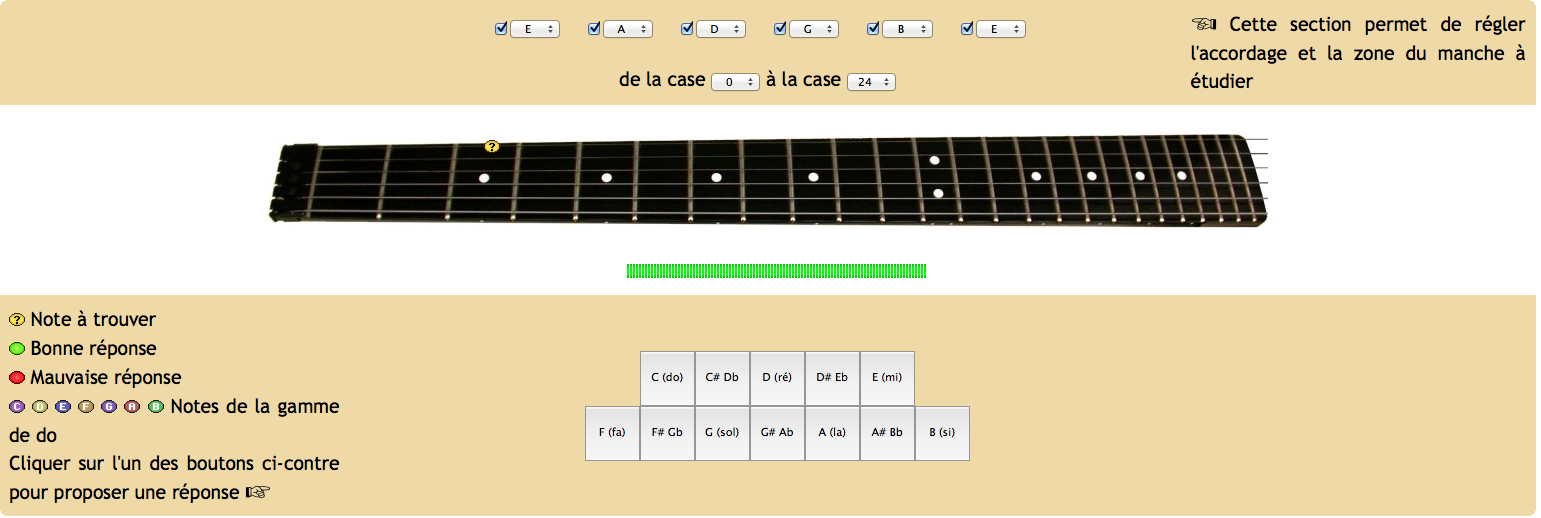
\includegraphics[width=10.5cm]{images/balezator_manche.png}
	\end{frame}

	\begin{frame}

		\frametitle{Lecture sur la portée}
			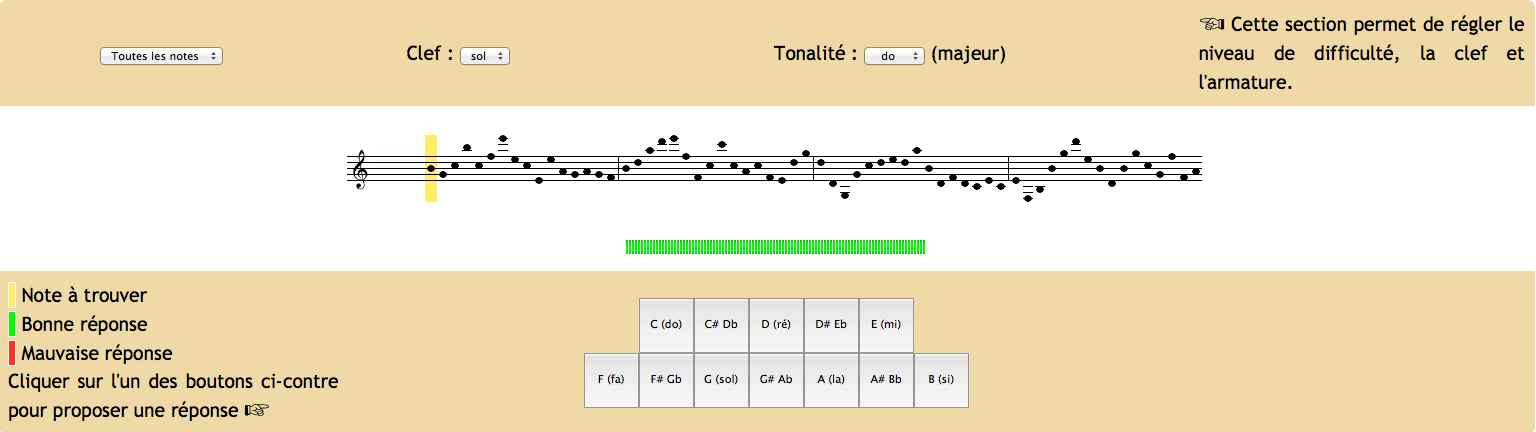
\includegraphics[width=10.5cm]{images/balezator_portee.png}

	\end{frame}



	% *** iBalezator ***
	\subsection{iBalezator}

	\begin{frame}
		\frametitle{Mode manche/clavier}
			MANCHE CLAVIER
	\end{frame}

	\begin{frame}
		\frametitle{Mode portée/manche}
			PORTEE MANCHE
 
	\end{frame}



	% *** Résumé des réunions précédentes ***
	\subsection{Résumé des réunions précédentes}

	\begin{frame}
		\frametitle{Réunions précédentes}
      		\framesubtitle{Points fondamentaux}
	\begin{itemize}
		\item Point 1 	
		\item Point 2
	\end{itemize}

	\end{frame}

